%-------------------------------------------------------------------------------
% File: software_architecture.tex
%       Part of StockSim project documentation.
%       See main.tex for further information.
%-------------------------------------------------------------------------------
\chapter{Software Architecture}
In this section the general software architecture of the application is
presented.\\
StockSim is a Java multi-module Maven application written using the IntelliJ
IDEA IDE.\\
We opted for a multi-module approach so that logically independent modules of
the applications could be kept separated and better maintained. This allowed
\begin{itemize}
    \item each of us to focus on the development of a particular module;
    \item to avoid code replication.
\end{itemize}
Furthermore, we decided to follow a feature-oriented development process and the
modularity of the project helped us code with more ease and efficiency.\\
\\
The entire codebase can be found at \url{https://github.com/rambodrahmani/stocksim}.
\section{Maven Multi-Module Structure}
The application consists of three modules: \texttt{Client}, \texttt{Server} and
\texttt{Library}.\\
The \texttt{parent} \texttt{.pom} defines the parent module Stocksim, with all
the dependencies and build settings that are common to the child modules.\\
\begin{lstlisting}[basicstyle=\footnotesize,language=Java,numbers=left,
    numberstyle=\footnotesize,numbersep=4pt,frame=single]
<?xml version="1.0" encoding="UTF-8"?>
<project xmlns="http://maven.apache.org/POM/4.0.0"
         xmlns:xsi="http://www.w3.org/2001/XMLSchema-instance"
         xsi:schemaLocation="http://maven.apache.org/POM/4.0.0 http://maven.apache.org/xsd/maven-4.0.0.xsd">
    <modelVersion>4.0.0</modelVersion>
    <groupId>it.unipi.lsmsdb.workgroup4</groupId>
    <artifactId>Stocksim</artifactId>
    <packaging>pom</packaging>
    <version>1.0</version>

    <!-- child modules -->
    <modules>
        <module>Client</module>
        <module>Server</module>
        <module>Library</module>
    </modules>

    [...]
\end{lstlisting}
Each child module has its own \texttt{.pom} file, necessary for the building
process and for keeping track of all the required dependencies.\\
\begin{lstlisting}[basicstyle=\footnotesize,language=Java,numbers=left,
    numberstyle=\footnotesize,numbersep=4pt,frame=single]
<?xml version="1.0" encoding="UTF-8"?>
<project xmlns="http://maven.apache.org/POM/4.0.0"
         xmlns:xsi="http://www.w3.org/2001/XMLSchema-instance"
         xsi:schemaLocation="http://maven.apache.org/POM/4.0.0 http://maven.apache.org/xsd/maven-4.0.0.xsd">
    <parent>
        <artifactId>Stocksim</artifactId>
        <groupId>it.unipi.lsmsdb.workgroup4</groupId>
        <version>1.0</version>
    </parent>

    <!-- child module -->
    <modelVersion>4.0.0</modelVersion>
    <artifactId>Server</artifactId>
    <packaging>jar</packaging>

    <!-- dependencies -->
    <dependencies>
        <dependency>
            <groupId>it.unipi.lsmsdb.workgroup4</groupId>
            <artifactId>Library</artifactId>
            <version>1.0-SNAPSHOT</version>
            <scope>compile</scope>
        </dependency>
        <dependency>
            <groupId>it.unipi.lsmsdb.workgroup4</groupId>
            <artifactId>Library</artifactId>
            <version>1.0</version>
            <scope>compile</scope>
        </dependency>
    </dependencies>

    [...]
\end{lstlisting}
For the full content of the \texttt{.pom} files please refer to Appendix A.
\subsection{Library}
The \texttt{Library} module, contains the database APIs both for MongoDB and
Apache Cassandra, together with the YahooFinance API and some utility functions.
The \texttt{Library} module was created in order to avoid code replication. The
\texttt{Client} and \texttt{Server} module relay on the APIs implemented in this
module.\\
It has the following structure:
\vspace{0.2cm}
\dirtree{%
.1 LIBRARY.
.2 src.
.3 main.
.4 java.
.5 it.unipi.lsmsdb.stocksim.lib.
.6 database.
.7 cassandra.
.7 mongoDB.
.6 util.
.6 yfinance.
}
\vspace{0.2cm}
\noindent The \texttt{database} package contains the two APIs we wrote for the
interaction with Apache Cassandra and MongoDB.\\
The \texttt{yfinance} package contains the API used to retrieve data from
Yahoo Finance. After trying some of the offered APIs, we decided to implement
our own from scratch.\\
The \texttt{util} package contains some utilities functions, such as the ones 
used to set the log level both for Apache Cassandra and MongoDB, and our custom
argument parser derived from \texttt{Apache Commons CLI} used to parse command
line arguments for both StockSim Server and StockSim Client.
\begin{figure}[H]
\begin{subfigure}{.3\textwidth}
  \hspace{-3.0cm}
  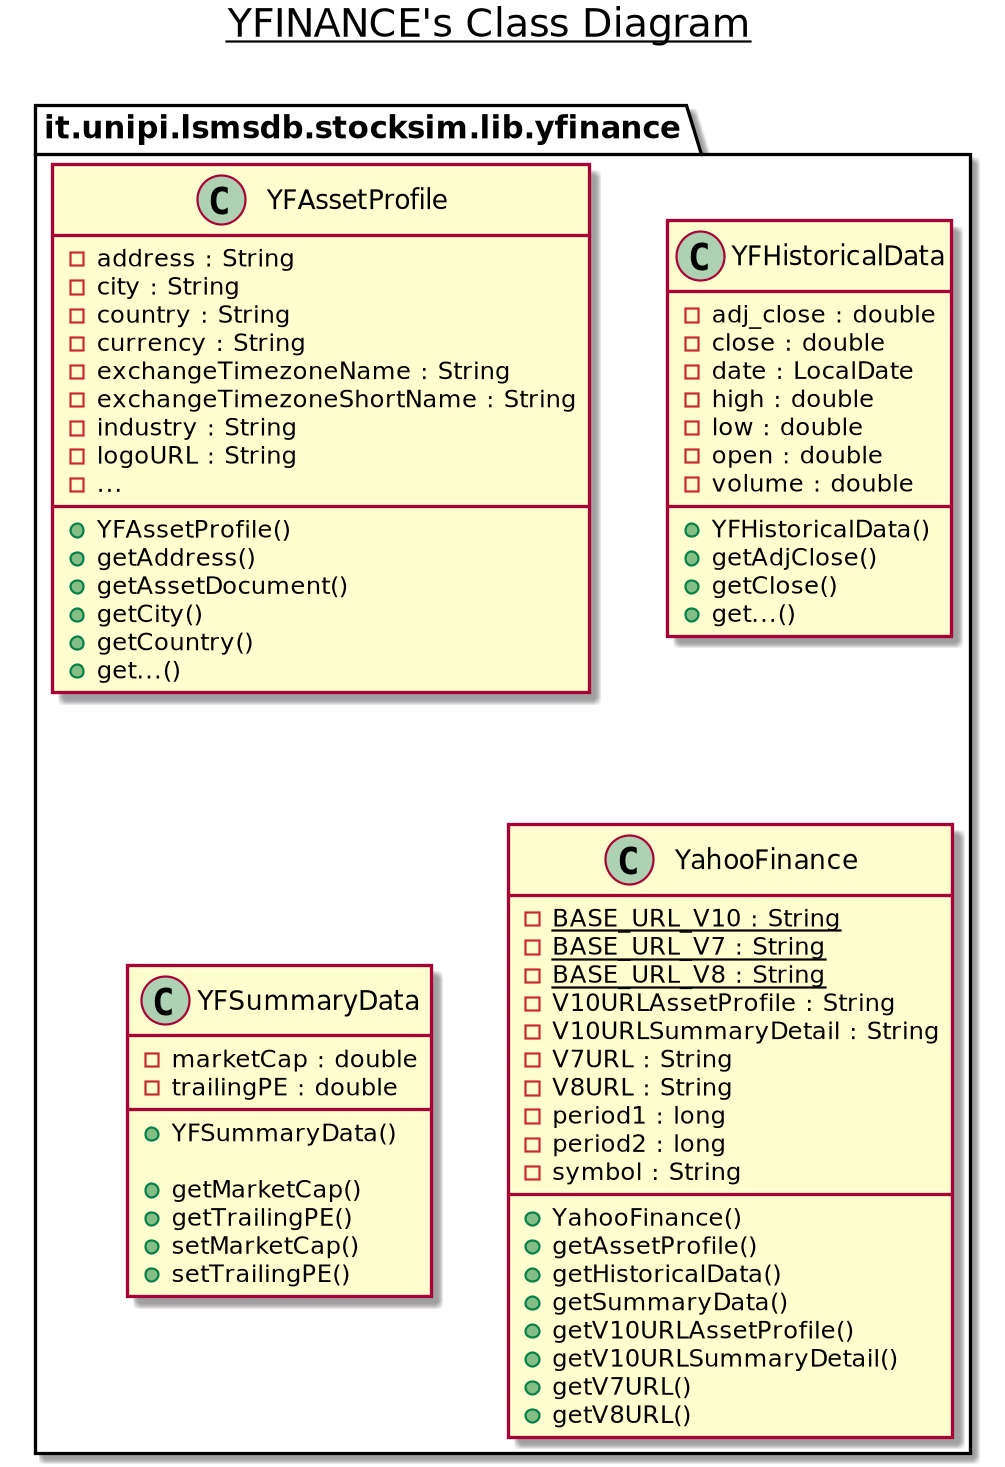
\includegraphics[scale=0.16]{plantuml/library/yfinance.png}
\end{subfigure}%
\hspace{-1.0cm}
\begin{subfigure}{.3\textwidth}
  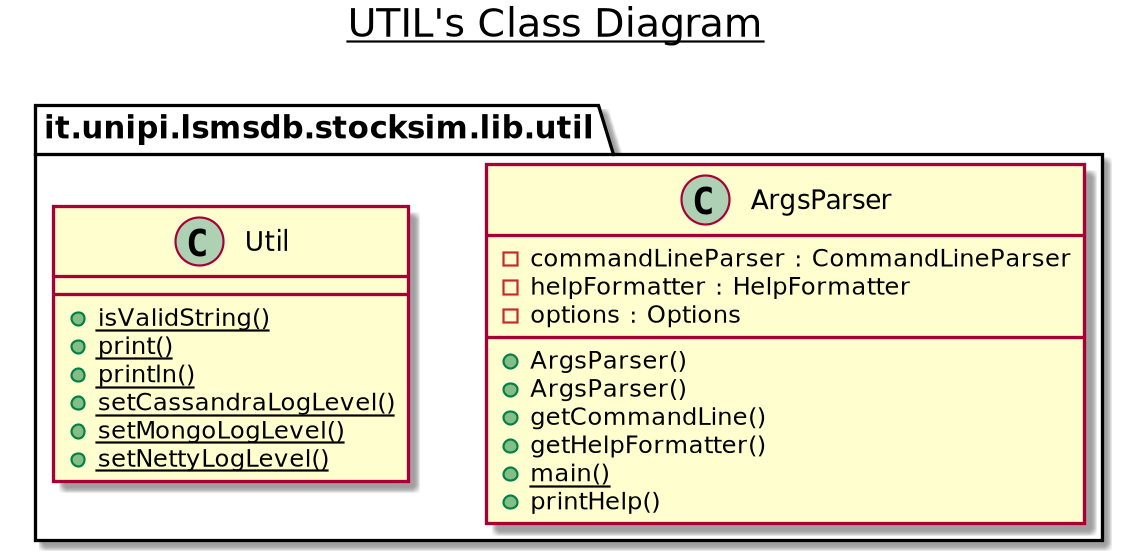
\includegraphics[scale=0.2]{plantuml/library/util.png}
\end{subfigure}
\hspace{4.0cm}
\begin{subfigure}{.3\textwidth}
  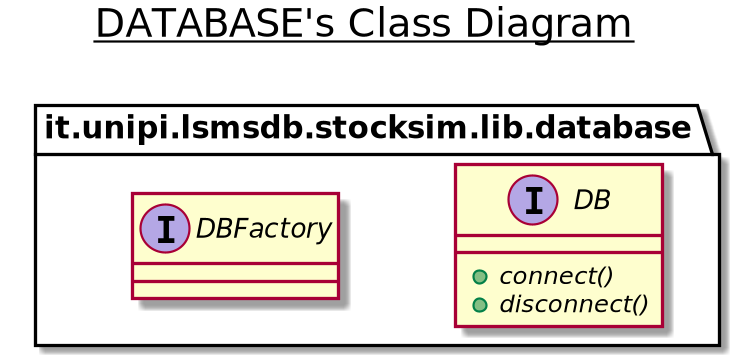
\includegraphics[scale=0.2]{plantuml/library/database.png}
\end{subfigure}
\end{figure}
\begin{figure}[H]
\begin{subfigure}{.5\textwidth}
  \hspace{-3.0cm}
  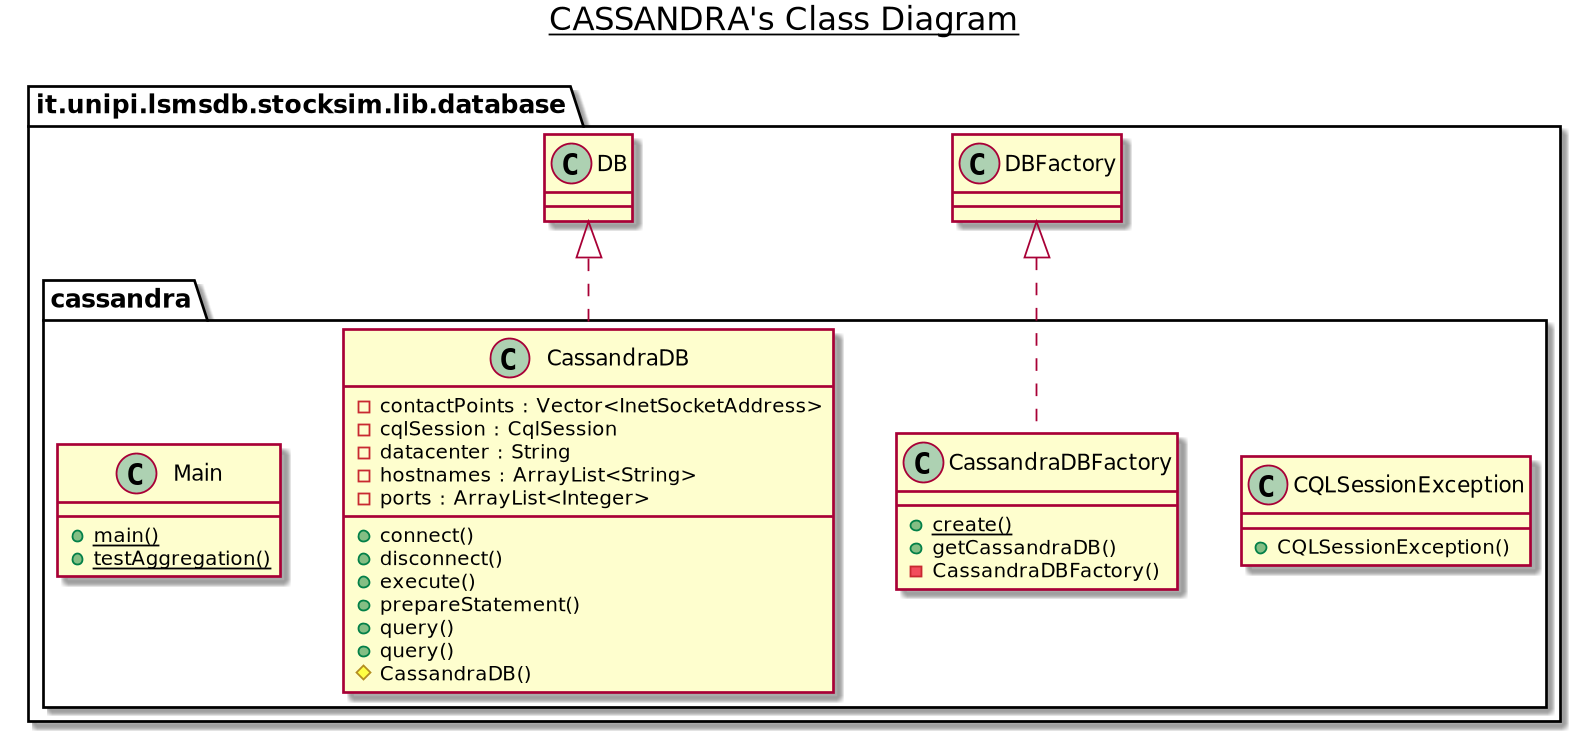
\includegraphics[scale=0.2]{plantuml/library/cassandra.png}
\end{subfigure}%
\hspace{1.0cm}
\begin{subfigure}{.5\textwidth}
  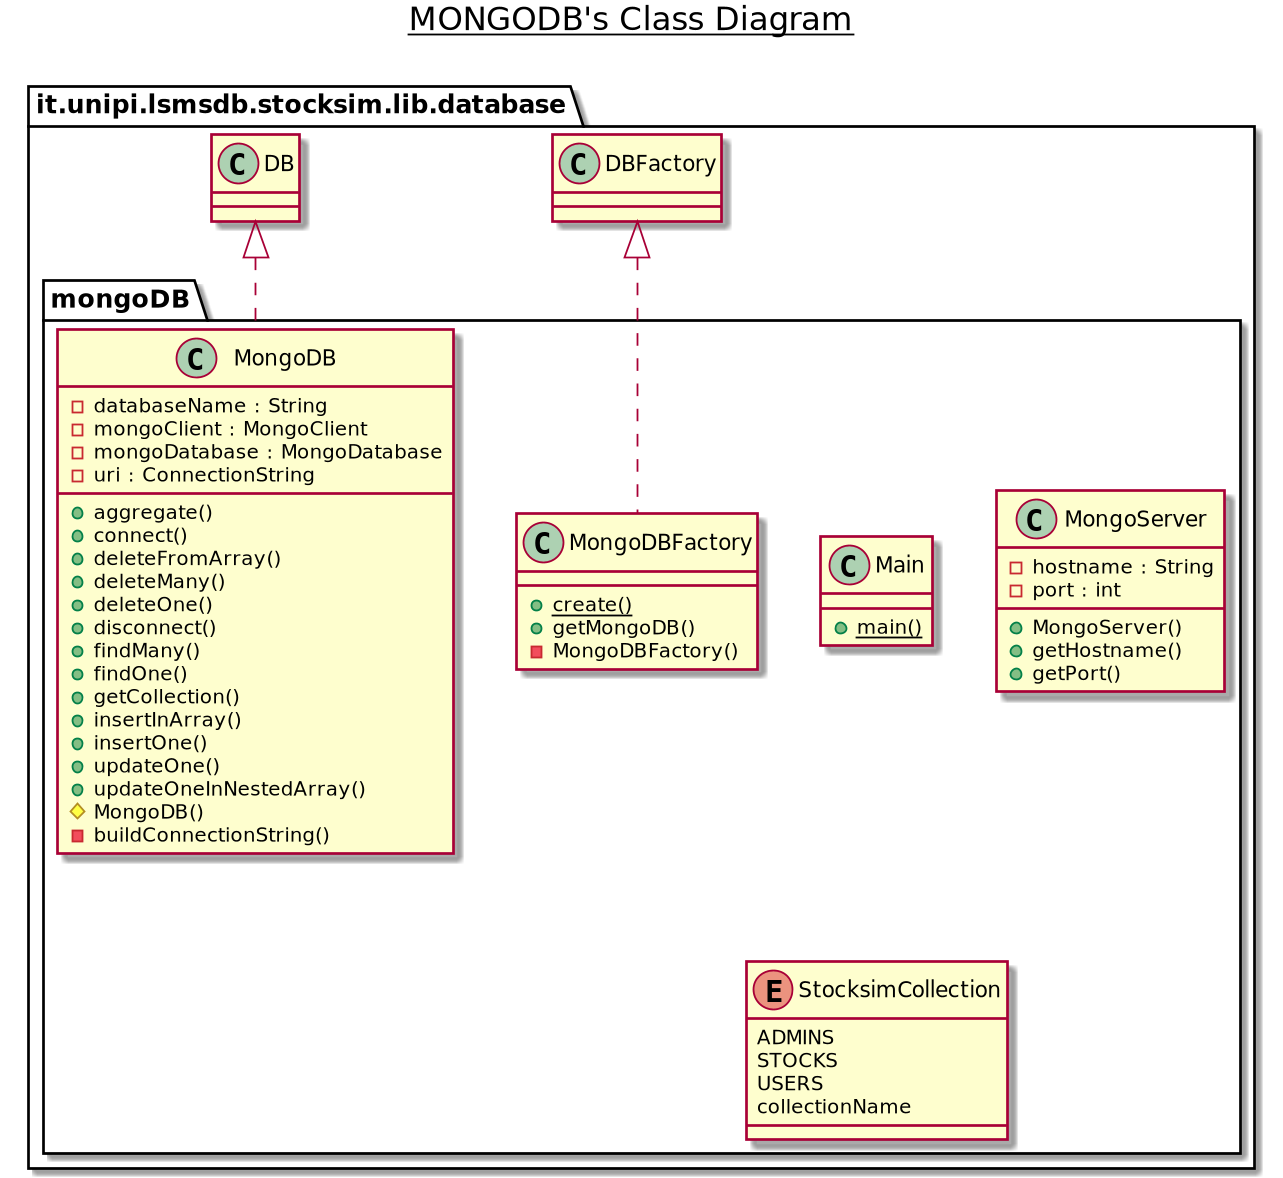
\includegraphics[scale=0.2]{plantuml/library/mongoDB.png}
\end{subfigure}
\caption{Library Module UML sample Diagrams}
\end{figure}
\subsection{Client}
The Client module contains the StockSim Client implementation. This program is
intended to be distributed to end users.\\
It has the following structure:
\vspace{0.2cm}
\dirtree{%
.1 CLIENT.
.2 src.
.3 main.
.4 java.
.5 it.unipi.lsmsdb.stocksim.client.
.6 admin.
.6 app.
.6 charting.
.6 database.
.6 user.
.3 resources.
}
\vspace{0.2cm}
\noindent The \texttt{app} directory contains the \texttt{Client.java} class
with the entry point for the application.\\
Since the StockSim Client program was thought to be executed in two different
running modes (namely \texttt{admin} or \texttt{user} mode), the \texttt{admin}
and \texttt{user} packages contain the implementation of the functionalities
available to the user in these two different running modes.
The \texttt{database} directory contains the classes necessary for the
connection management and the interaction with MongoDB and Apache Cassandra.
Also here you can find classes intended for storing the retrieved data.\\
The \texttt{charting} directory contains an API for the \texttt{JFreeChart}
library, used by the Client to create charts of various types.
\begin{figure}[H]
	\begin{center}
        \hspace*{-3.3cm}
		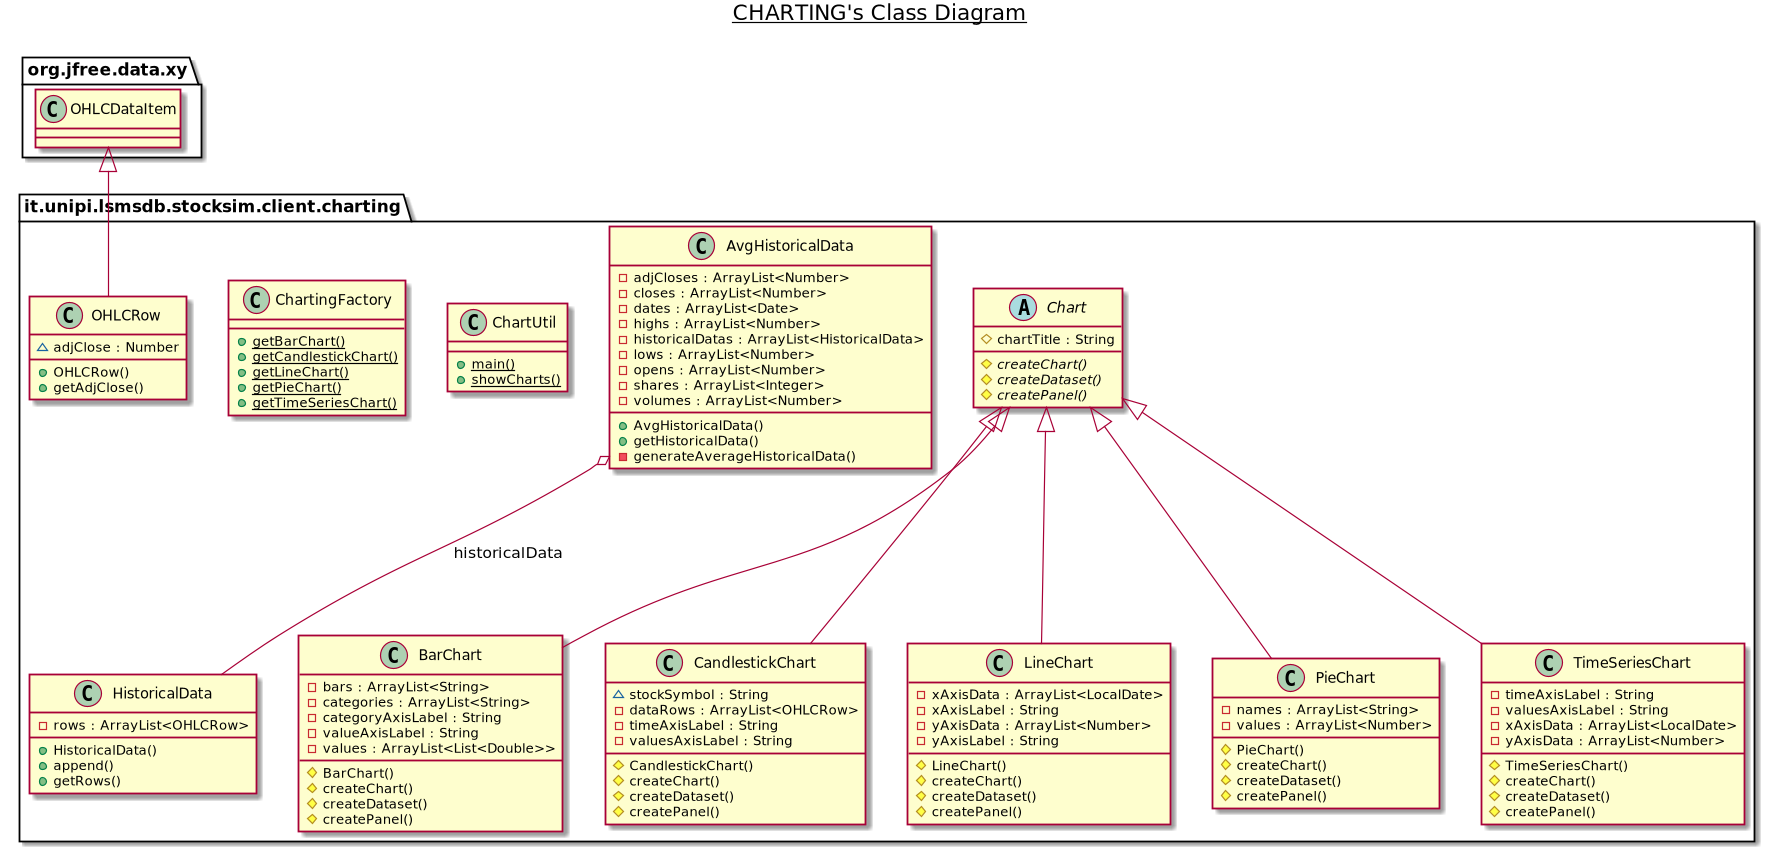
\includegraphics[scale=0.337]{plantuml/client/charting.png}
		\caption{Client charting package UML Diagram as sample}
	\end{center}
\end{figure}
\subsection{Server}
The Server module represents the StockSim Server program which takes care of
keeping the data updated and consistent.\\
It is not supposed to be distributed: it should be always running in order to be
able to retrieve the historical data prices relative to the latest trading
session.\\
The Server module has the following structure:
\vspace{0.2cm}
\dirtree{%
.1 SERVER.
.2 src.
.3 main.
.4 java.
.5 it.unipi.lsmsdb.stocksim.server.
.6 app.
.7 Server.java.
.7 ServerUtil.java.
.6 database.
.7 CassandraQueryBuilder.java.
.7 DBManager.java.
}
\vspace{0.2cm}
\noindent The \texttt{app} package contains the class with the entry point for
the application.\\
The \texttt{database} package contains the classes necessary for the interaction
with the databases.
\begin{figure}[H]
\begin{subfigure}{.5\textwidth}
  \hspace{-2.0cm}
  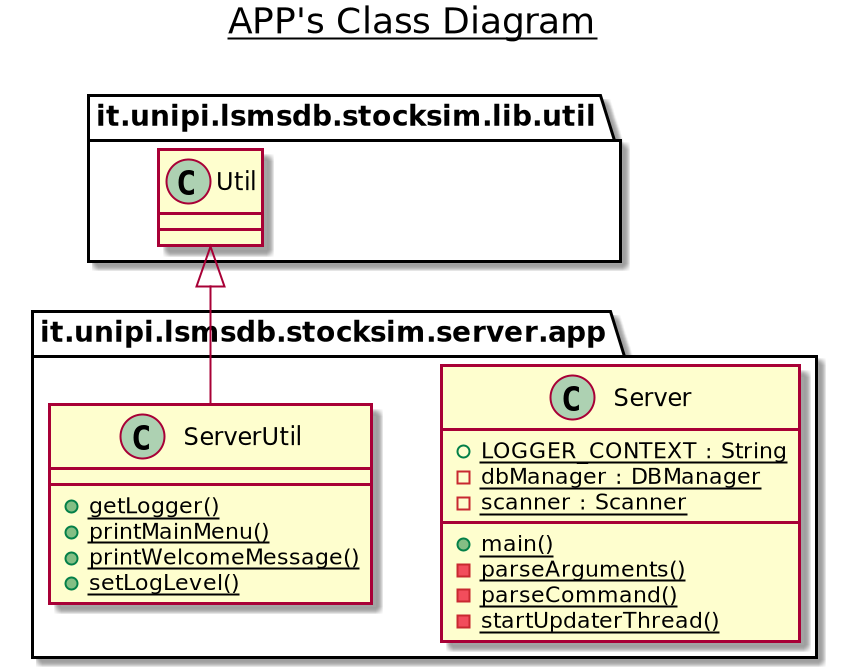
\includegraphics[scale=0.2]{plantuml/server/app.png}
\end{subfigure}%
\hspace{-2.0cm}
\begin{subfigure}{.5\textwidth}
  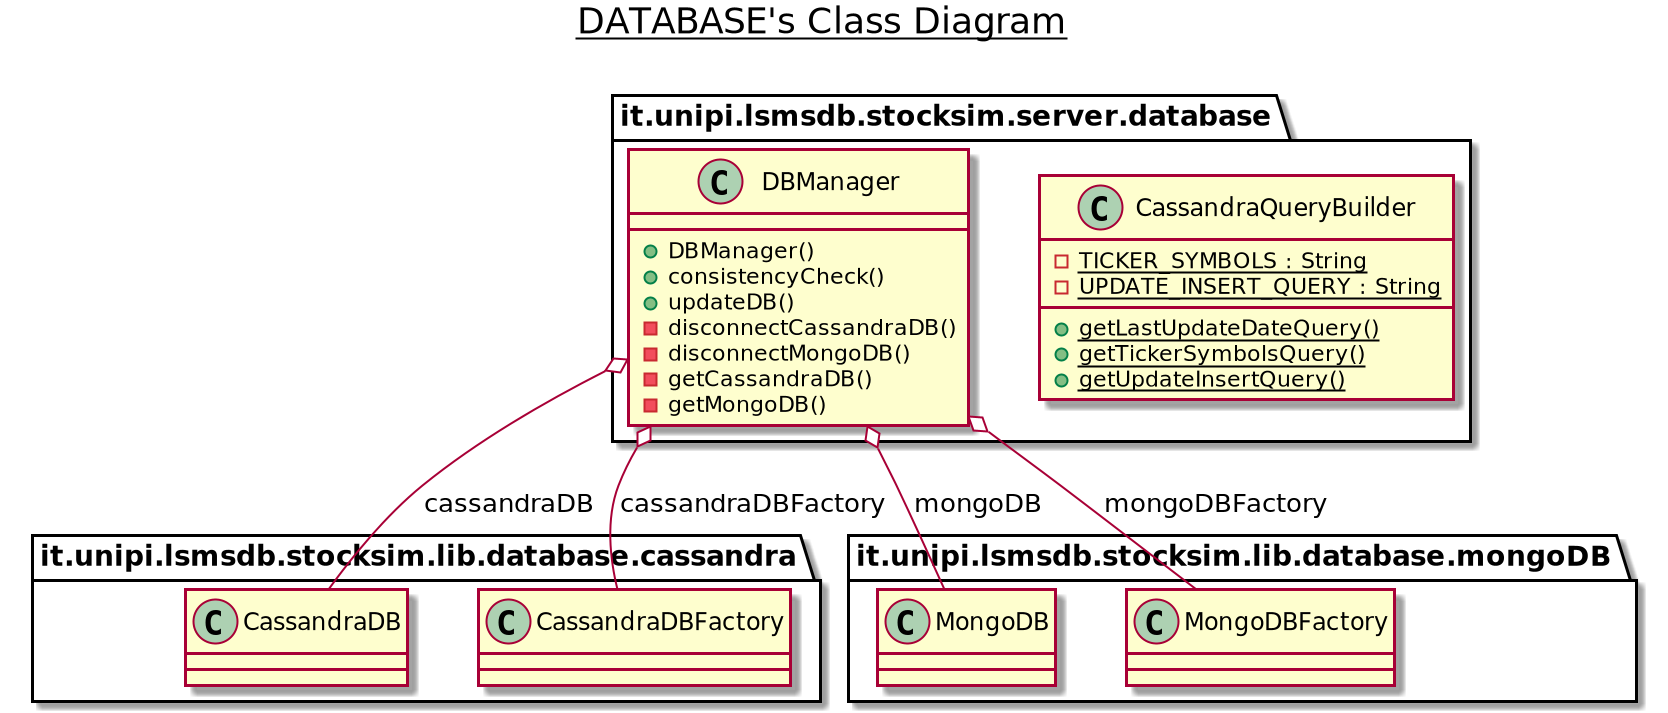
\includegraphics[scale=0.2]{plantuml/server/database.png}
\end{subfigure}
\caption{Server Module UML sample Diagrams}
\end{figure}
\section{Apache Maven Compiler Plugin}
The Compiler Plugin is used to compile the sources of the project.
\vspace{0.2cm}
\begin{lstlisting}[basicstyle=\footnotesize\ttfamily,language={},numbers=left,
keepspaces=true,tabsize=4,numberstyle=\footnotesize,numbersep=8pt,frame=single]
$ mvn package
\end{lstlisting}
\vspace{-0.3cm}
The command line will print out various actions, and end with the following:
\vspace{0.2cm}
\begin{lstlisting}[basicstyle=\footnotesize\ttfamily,language={},numbers=left,
keepspaces=true,tabsize=4,numberstyle=\footnotesize,numbersep=8pt,frame=single]
[INFO] ------------------------------------------------------------------------
[INFO] Reactor Summary for Stocksim 1.0:
[INFO] 
[INFO] Stocksim ........................................... SUCCESS [  0.001 s]
[INFO] Library ............................................ SUCCESS [  0.820 s]
[INFO] Client ............................................. SUCCESS [  6.287 s]
[INFO] Server ............................................. SUCCESS [  5.337 s]
[INFO] ------------------------------------------------------------------------
[INFO] BUILD SUCCESS
[INFO] ------------------------------------------------------------------------
[INFO] Total time:  12.514 s
[INFO] Finished at: 2021-01-24T12:58:10+01:00
[INFO] ------------------------------------------------------------------------
\end{lstlisting}
Thanks to the proper configuration in the \texttt{.pom} file of each module,
the following files are produced
\vspace{0.2cm}
\dirtree{%
.1 Stocksim.
.2 Library.
.3 target.
.4 Library-1.0.jar.
.2 Client.
.3 target.
.4 Client-1.0.jar.
.4 Client-1.0-jar-with-dependencies.jar.
.2 Server.
.3 target.
.4 Server-1.0.jar.
.4 Server-1.0-jar-with-dependencies.jar.
}
\vspace{0.2cm}
\noindent The \texttt{jar-with-dependencies} \texttt{.jar} files provide all-inclusive
Java Archives which can be used to execute the StockSim Server and the StockSim
Client programs.
